\chapter{Benchmark Tool}
\begin{itemize}
    \item Vysvětlit usecase
    \item Design
    \item Použité technologie
\end{itemize}
To facilitate future evaluations of the models on new datasets, we have
"wrapped" the raw code used for our evaluation into a \bld{graphical user
    interface (GUI) application}. We have decided to implement the GUI as a
bld{web application}. This approach naturally solves the cross-platform (in
terms of operating systems) compatibility. On top of that, developing native
desktop applications can be very tedious; therefore, we have made this decision.
We believe that "running" a web application is more natural today.

As we mentioned, the GUI (\bld{frontend}) is implemented as a web application
with a JavaScript framework. The application's logic (\bld{backend}) is
implemented separately in Python and is accessed by HTTP requests. In the
following sections, we describe the application's design and implementation
details.

\section{Design}
The application's primary purpose is to train and evaluate selected models with
user-specified parameters on an arbitrary object detection dataset. We describe
the typical scenario of the user interaction with the application below:
\renewcommand{\theenumi}{\arabic{enumi}}
\begin{enumerate}
    \item The user uploads a new dataset or selects an old one. He can
          optionally define a split ratio by which the dataset will be split
          into training, test, and validation set.
    \item The user selects models to evaluate.
    \item The user sets models' parameters.
    \item The user initiates the training.
    \item The user then observes the results and eventually downloads the
          evaluation data.
\end{enumerate}
As we can see, the process can be split into a sequence of steps. Therefore, in
terms of the GUI design, we took inspiration from the layout of "setup wizards" (see Figure \ref{fig:wizard}).
At each step, only the relevant information is visible. The user can only go to
the previous or next step (if the user provides all the necessary information).

\begin{figure}[h]
    \centering
    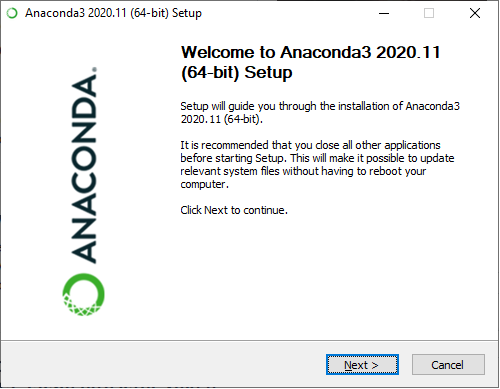
\includegraphics[width=0.65\linewidth]{Sources/Figures/anaconda.png}
    \caption{An example of a setup wizard.}
    \label{fig:wizard}
\end{figure}

The frontend communicates with the backend through the HTTP application
programming interface (API) composed of uniform resource identifier (URI)
endpoints. The API will consist mainly \texttt{GET} and \texttt{POST} requests.
For example, if we would like to retrieve a list of datasets, we would send a
GET request to a URI of the form similar to \texttt{<api\_address>/datasets}.

\section{Implementation}
Fortunately, we could implement this layout with ease by using a Material Design
Framework Vuetify that includes a "stepper" component that corresponds to the
design as mentioned above.